\begin{frame}{Song song hoá quá trình khuếch tán}
\begin{itemize}
    \item Sử dụng \emph{thứ tự đỏ-đen}
    \begin{figure}[H]
        \centering
        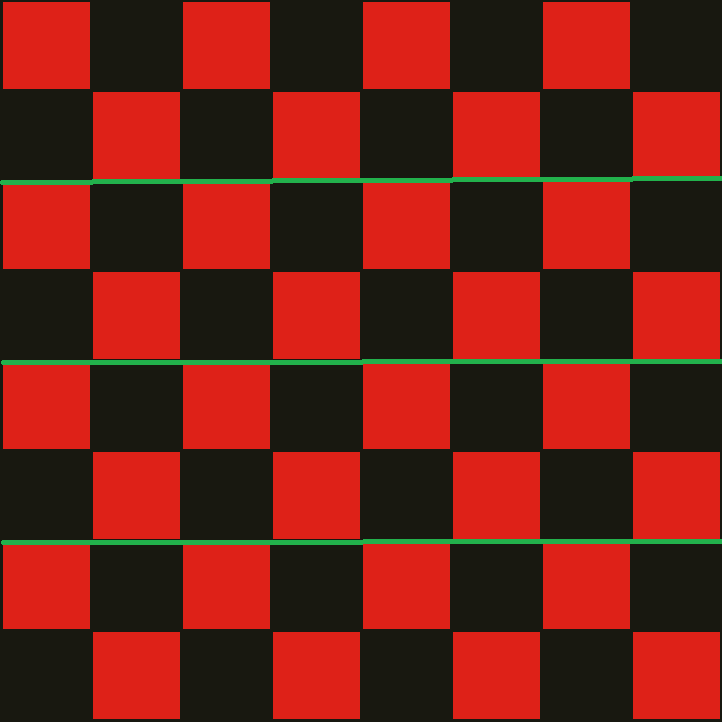
\includegraphics[width=22mm]{img/red-black-grid.png}
    \end{figure}
	\item Tại mỗi bước lặp, cập nhật các ô màu \emph{đỏ} trước, sau đó cập nhật các ô màu \emph{đen}.
	\item Các ô cùng màu được cập nhật song song theo \emph{thứ tự hàng}.
	\item \emph{Nhận xét:} Các ô màu đỏ được cập nhật hoàn toàn dựa vào kết quả ở bước lặp trước, chỉ các ô màu đen được cập nhật theo đúng công thức \emph{SOR}.
\end{itemize}
\end{frame}